
\section{Nested Relational Model, Semistructured data and Streams}\label{sec:semistructured}
A data model is said to be \textbf{semistructured} if it relies on a fixed data model over which \textbf{no} constraints are imposed. Given this definition, we could now distinguish the \textbf{nested relational model} from the \textbf{XML data model}\index{XML|textbf}: even though both models rely on the relaxation of the 1NF\index{1NF} by allowing nested data representations as possible data values (thus allowing the representation of hierarchical data), the former model still requires the nested relations to be compliant to a given schema, while the latter does not. As a consequence, the first model still suffers from the ``data homogeneity'' problem addressed for the Relational Model in Section \vref{par:homog}, while the second does not. 

\begin{figure}[!hpt]
\lstinputlisting[language=XML,basicstyle=\ttfamily\small]{fig/02models/VendorSales.xml}
\caption{Representing the association between the \texttt{Vendors} and their \texttt{SalesOrder}s in Figure \ref{fig:instance} with an XML representation.}
\label{fig:semistructXML}
\end{figure}


\begin{example}
	As we could see in Figure \ref{fig:semistructXML}, XML achieves the 1NF relaxation through the definition of \textit{tags}: a tag is a construct beginning with the character ``<'' and ending with ``>'': all the data is contained between the \textit{start tag} (e.g., ``\texttt{<Database>}'') and the \textit{end tag} (e.g., ``\texttt{</Database>}''), that could cointain either textual elements or other tags. To each tag, some properties and values could be associated (e.g. the tag ``\texttt{<Vendor id=\textquotedbl001\textquotedbl>\dots </Vendor>}'' contains a property \texttt{id} with value \texttt{001}). An empty tag (e.g., ``\texttt{<salesOrder />}'') represents a tag containing no information. Table \ref{tab:semistructTable} provides the same representation for nested relations: in this case the nested data representation is represented by relations that could be used as valid values for some attributes (e.g., \texttt{salesOrder}), provided that the relation has a fixed schema. The empty tag could be represented by either a \texttt{NULL} value or an empty relation. 
	
	A graphical representation of such tree is provided in Figure \ref{fig:semistructXMLTree} in the footsteps of \cite{Magnani06}. Please note that such alternative representation does not consider the tag's attributes like ``id'', and only provides labeless edges. A more complete XML data model representation in this regard is provided by Lu \cite{Lu2006}, also allowing to integrate relational data with XML and Object Oriented databases.
\end{example}

\begin{table}[!t]
\centering
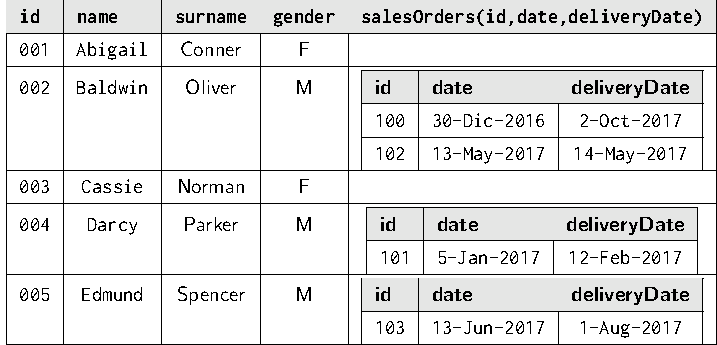
\includegraphics[scale=0.9]{fig/02models/01nestedaggr}
\caption{Representing the association between the \texttt{Vendors} and their \texttt{SalesOrder}s in Figure \ref{fig:instance} with a nested tabular representation. Each attribute containing a nested relation exposes both the name of the attribute and the schema associated to the relations that it contains. }
\label{tab:semistructTable}
\end{table}\begin{figure}[!t]
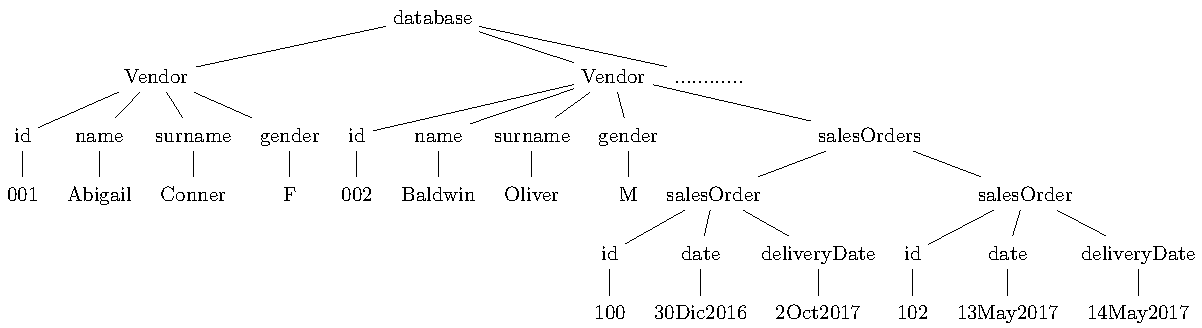
\includegraphics[scale=0.7]{fig/02models/02anestedasTree.pdf}
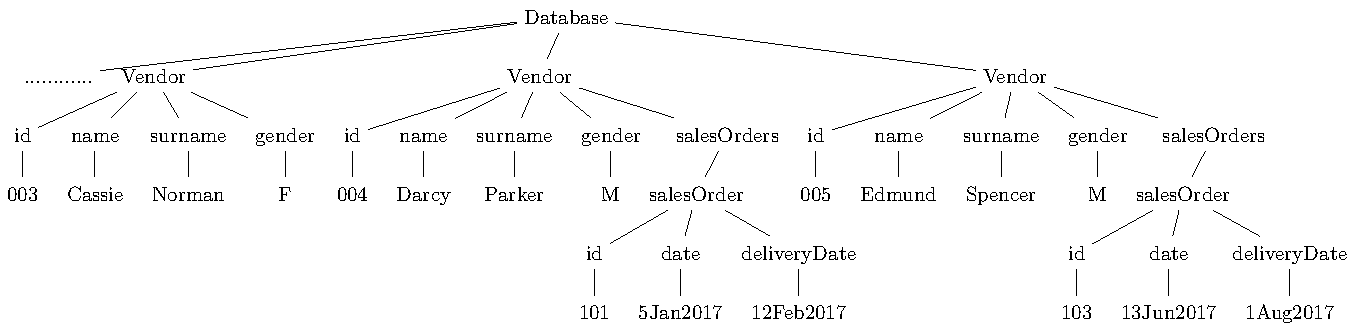
\includegraphics[scale=0.63]{fig/02models/02bnestedasTree.pdf}
\caption{Representing the association between the \texttt{Vendors} and their \texttt{SalesOrder}s with an tree representation of Figure \ref{fig:semistructXML}. Please note that the two trees represent the same XML document, that has been here split in two parts due to page size and readability limitations. The representation of choice is the one provided in \cite{Magnani06}, where no tag attributes are considered. The XML's empty tags are removed since they are not supported by the data model.}
\label{fig:semistructXMLTree}
\end{figure}

The flexibility of the XML representation is also evident by the fact that one single tag can contain multiple tags with the same name, while the nested relational model only allows one single attribute per nested relation. As a consequence, the XML model generalizes the Object model represented in Definition \vref{def:mof} because within that definition, the attribute-value association is implicitly represented by a map while, in this case, such association can be represented with a multimap.

Data models having no fixed schema could be always be associated to a schema in a later step: for example, tag schema could be externally validated through \textbf{XML Schema}\footnote{Other languages that could be used to express XML schemas are RelaxNG and DTD, even though such languages do not use the XML syntax.} \cite{VlistXS}, expressing such constraints within the same XML data representation. As a result, while the XML data model is widely adopted due to its flexibility in web technologies, the nested relational model is not, even though it is adopted for providing multidimensional view of structured data (thus, homogeneous) as in Pentaho \cite{Pentaho} and JasperServer \cite{Parra}. The reason why the nested relations are preferred for visualizing nested multidimensional data is evident by comparing the XML representation in Figure \ref{fig:semistructXML} with the nested representation in Table \ref{tab:semistructTable}. XML is more verbose and less compact and intuitive than  the nested relational tables.



%% Il punto C scritto a mano è sbagliato.
%% TODO: la rappresentazione annidata in tabelle è molto più compatta di quella XML, ma non permette di rappresentare liberamente tutti gli XML possibili.

\begin{figure}
	\centering
	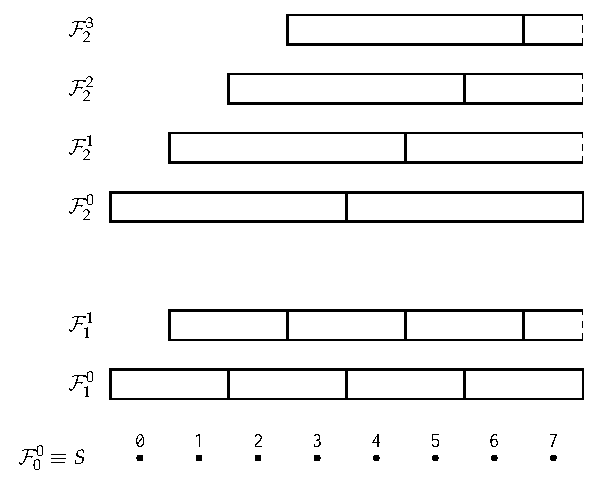
\includegraphics[scale=0.7]{fig/02models/06stream}
	\caption{A representation of an \textit{incremental feature extraction} scenario, where the window size is $w=2$ and the update rate is $T=1$. If we use $\alpha$ as the sum function, then $\mathcal{F}_1^0[0]=1$ and $\mathcal{F}_2^0[0]=6$, where $\mathcal{F}_2^0[0]=\mathcal{F}_1^0[0]+\mathcal{F}_1^0[1]=(0+1)+(2+3)$.}\label{fig:stream}
\end{figure}
Last, we must also observe that the previous nested relational models and semistructured models do not allow a complete representation of the \textbf{stream data model}. This data model is an extension of collection representations \cite{LawWZ04,ArasuW04}, where the  incoming stream $S[0,\dots,n-1]$ is represented as a collection of $n$ values. On top of such stream, we may create features $\mathcal{F}_{j+1}^T$ representing data at a given resolution $j$, which it may be sampled after a (possibly zero) update rate $T$ \cite{BulutS07}. Each value  $\mathcal{F}_{j+1}^T[i]\in \mathcal{F}_{j+1}^T$ may be computed from a finer data resolution $\alpha(\mathcal{F}_{j}^{T\mod{w^j}}[iw,\dots,(i+1)w-1])$, where $\alpha$ is an abstraction function \cite{Johnson2011} allowing dimensionality reduction for acquiring higher level information \cite{BulutS07}. 

\begin{example}
Figure \ref{fig:stream} provides an example of a data stream where $\alpha$ is the sum function over naturals. This implies that each possible sub-collection $\mathcal{F}_{j}^{T\mod{w^j}}[iw,\dots,(i+1)w-1]\subset \mathcal{F}_{j}^{T\mod{w^j}}$ must both represent a value, and have an associated value, too. In particular, such feature is missing in current nested and document based data models, thus making impossible the definition of structural aggregations as required by current MOLAP systems (see Example \vref{ex:inaggr}). 

Last, please observe that each data element can be part of different multiple stream representations. For example, both raw data and aggregated data are contained in multiple coarser representations. In the first case, $S[1]=1$ is contained in both $\mathcal{F}_1^0[0]$ and $\mathcal{F}_1^1$; in the second case, $F_1^0[1]$ is contained in both $\mathcal{F}_2^0[0]$ and $\mathcal{F}_2^2[0]$.
\end{example}


\subsection{Query languages}
It has been already proved that any nested relational query expressed in the nested calculus could be mapped into a relational algebra query run over a flattened representation of the nested relational algebra  \cite{ParedaensG92}. As a result, such nested calculus benefits from the same rewriting rules presented within the relational model, and hence benefits from the same query optimization operations. Since the relational algebra has been also extended to XML trees \cite{Lu2006}, then as a result we have that even such algebras take advantage of such rewriting rules \cite{Magnani06}. Despite the interest of data integration between structured and semi-structured that such query language made feasible, none of the aforementioned algebras have been implemented yet in real systems.

However, traversing query languages over one single representation and over semistructured data have been more successful: in particular, \textbf{XPath}\index{XPath|textbf} \cite{xpath31} is very used within other semistructured query languages, such as \textbf{XQuery} \cite{XQuery} and \textbf{XSLT} \cite{Tidwell},  transforming semistructured documents in order to obtain other documents, represented in any format. %\todo{Aggiungere un esempio di questi linguaggi?} 
In the footsteps of \cite{Magnani06}, we're going to analyse a minimal subset of XPath, merely concerning the path traversal, thus discarding all the axis notation and the selection predicates. 


\begin{definition}[Minimal XPath]
	\label{def:minxpath}
	A minimal XPath expression $\texttt{<}\mu\texttt{XPath}\texttt{>}$ is formed by a concatenation of traversal operator \texttt{<c>}, that can be either \texttt{/} (direct descendant) or \texttt{//} (any node contained at any depth) to which a collection selector (\texttt{<s>}) may be applied (e.g. \texttt{/$^{\mstr{Tag}}$}, which means to select the nodes directly descendant from root contained in the \texttt{Tags} collection). 
	\[\texttt{<s>}:=\varepsilon\; |\; \star\;|\;\texttt{[name]}\]
	\[\texttt{<c>}:=\texttt{/}^\texttt{<s>}\;|\;\texttt{//}^\star\]
	\[\texttt{<}\mu\texttt{XPath}\texttt{>} :=\texttt{<c>}\texttt{<s>}\;|\;\texttt{<c>}\texttt{<s>}\texttt{<}\mu\texttt{XPath}\texttt{>}\]
\end{definition}

The semantics associated to such query language \cite{Wadler00} returns the forest (tree collection) that is reached after the stepwise evaluation of the XPath expressions.

%On the other hand, The relaxation of the 1NF allows to also navigate the data structure in depth: Concerning query languages for semi-structured data, some languages have been proposed: : the first one implements traversal queries
%that are used in the second language, which is functional and expression-oriented.  \texttt{[TODO]}

\subsection{Representation problems}\label{sec:semireprproblems}
Given that property graphs do not relax 1NF\index{1NF}, they do not allow nested representations. Therefore, we cannot say that they provide a better representation than the data models that have been now presented, but we can only say that are complementary models. As a consequence, this section is going to be later on used as a set of requirements that general semistructured data models must satisfy for solving the representation problems. The resulting data model will be presented in a separate chapter (Chapter \vref{sec:datamodelglit}).

\paragraph*{Semantic Overloading} Both models suffer from  semantic overloading: while the motivation for the nested relational model could be  found in Section \vref{subsec:semanticoverloadrel}, the XML model suffers from this problem because it uses tags for both expressing entities (e.g., \texttt{Vendor}), properties (e.g., \texttt{name}, \texttt{surname}) to which values could be associated, and nesting components (e.g., \texttt{salesOrders}). This problem is practically solved within the proposed property graph model, where labels $l\in L$ belong to a different set than attributes $a\in A$, and attributes could be not expressed in two possible different ways (e.g. tag attributes and tags containing values). On the other hand, the nested extension of the property graph model should allow to contain vertices and edges, as nested relations could contain other relations as values, as well as XML tags' contents could be other XML tags.

\paragraph*{Data Homogeneity} As previously discussed, only the nested relational model suffers from this representational problem because it still has an associated schema. As a consequence, each nested relational table could be expressed by a XML document, but not the other way around. As a consequence, within this thesis we're going to represent nested relations as nested tables.


\begin{table}[!t]
\centering
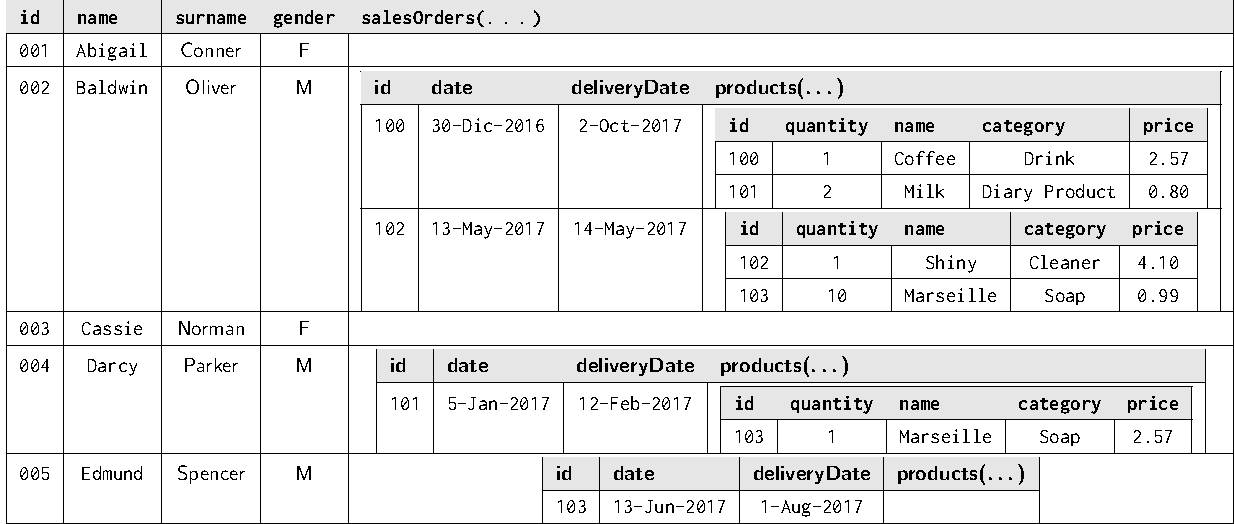
\includegraphics[scale=0.7]{fig/02models/02nestedaggrSales.pdf}
\caption{Extending the nested representation of Table \ref{tab:semistructTable} for showing the defect of the data representation over multiple nesting levels.}
\label{tab:semistructTableMultipleNest}
\end{table}
\paragraph*{Data Replication vs. Object Identity}
When nesting multiple relations at different levels, the need of univocally identified object becomes more evident. Let us observe Table \ref{tab:semistructTableMultipleNest}, extending the previous nested relation example. As  tuples describing the same entity (e.g., the product names \texttt{SPAM} having \texttt{id} \texttt{103}) appear in different places within the table, their price change requires a complete scan of the whole table. Update operations within these models are quite inefficient (update of multiple instances against an update of one single instance), therefore the nested relational data model could not be used for representing hierarchical data changing through time. Moreover, since the nested relational model also suffers from semantic overloading, the description of the entity \texttt{Product} now also depends on the \texttt{SaleOrder}'s quantity of ordered products.

To avoid data replication problems, direct value containment should be replaced by object identifier containment. At the time of the writing, nested graphs data models are represented by the former approach (e.g., GraphML \cite{graphml}), while our proposed data model is going to adopt the latter solution (Chapter \ref{cha:graphsdef}).
%As a consequence, vertices and edges shall not directly contain other vertices and edges as in the GraphML model  \cite{graphml}, but must only contain the reference (\textit{id}) to such vertices and edges, thus avoiding data replication problems. This solution is going to be adopted by our proposed data model depicted in Chapter \ref{cha:graphsdef}.


\subsection{Representing graphs}
Even if XML was originally designed to represent tree data structures, it could also  represent graphs through specific XML schemas. \textbf{GraphML} \cite{graphml} and \textbf{GXL} \cite{gxlgraphml}, which are based on the XML markup language, allow to express graphs, that could also contain other graphs (\textit{nested graphs}) inside some other vertices and edges. We're going to analyze and compare such data models with the one we propose in Section \vref{sec:datamodelglit}.


On the other hand, graphs could be also used to represent semistructured information, such as XML documents \cite{Lassila1999,GutierrezInclusion}. As well as XML, graphs could provide a syntactical representation (\textit{metadata}, see Chapter \ref{cha:dataintegration}) of the XML data: as a result, we could analyze how different authors choose to differently use the tags within some XML documents, and investigate which ``structural patterns'' have been used \cite{IorioHierarchy,BarabucciEARMARK}. 

This fact also suggests that graphs must belong to the \textit{semistructured data} family and that all semistructured data are able to describe both data and the meta-data level with the same description language, as well as describing query languages (compare the aforementioned XSLT query language in XML and GraphQL \cite{GraphLogAggr} pattern query language, which is expressed through graphs, like also another graph pattern query language \cite{n3} and some artificial intelligence one \cite{Goertzel2014}).

%In this case a Semantic Web Graph representation of such documents
%provides a ideal schema-independent data structure  that could be used in automatic reasoners such as \textbf{Jena} \cite{Jena} and \textbf{Pellet} \cite{Pellet} to extract the 
%structural informations.
\medskip